\section{Experiments}
\label{sec:experiments}

We analyze 11 of ScienceWorld's 30 task types (245 episodes); the 19 excluded types (63\%) lack actionable routing signal due to development contamination (5), taxonomic redundancy (7), or agent-floor performance (7). Taxonomically redundant tasks share identical action vocabularies, reward functions, and environmental dynamics, differing only in target entity; we retain one representative per family (Appendix~\ref{app:per-task}). This scope limits generalizability: conclusions apply to the included subset; increasing the 30-step budget might surface signal in excluded types (see Limitations). An anti-cherry-picking analysis confirms that death dominance holds in 18 of these 19 types, with a mean $\Delta\text{DR} = +38.2$\,pp exceeding the included tasks' $+28.7$\,pp (Appendix~\ref{app:per-task}). Extended validation at $n{=}20$ on five representative excluded tasks confirms this direction ($\overline{\Delta\text{DR}} = +32.0$\,pp; Appendix~\ref{app:extended-validation}). A reasoning-depth ablation ($n{=}120$) found no significant difference between internal strategy variants ($p > 0.26$; Appendix~\ref{app:ablations}). Prescreening used $n{=}5$ episodes per task type; directional consistency (18/19 types favoring deterministic) rather than point estimates drives the inclusion criterion.

\subsection{Death Avoidance Decomposition}
\label{sec:death-decomp}

\begin{figure}[t]
\centering
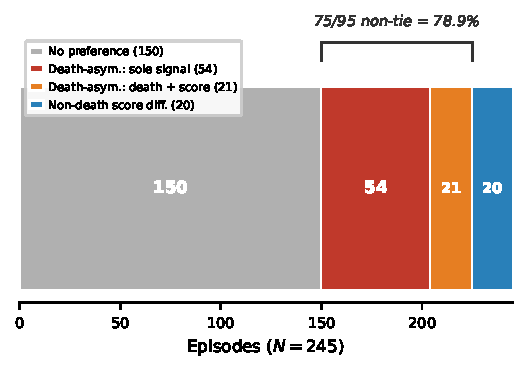
\includegraphics[width=\columnwidth]{figures/label_decomposition.pdf}
\caption{Episode-level label decomposition ($N{=}245$). Of 95 non-tie labels, 75 (78.9\%) arise from death asymmetry: 54 where death is the sole discriminator and 21 with co-occurring score differences. All 20 non-death labels originate from a single task type (\texttt{find-non-living-thing}).}
\label{fig:label-decomposition}
\end{figure}

Of the 95 non-tie routing labels (Figure~\ref{fig:label-decomposition}), 75 (78.9\%; 95\% CI: $[70.7\%, 87.0\%]$, episode-level bootstrap) arise from death asymmetry: the internal strategy triggers a catastrophic $-100$ penalty while the deterministic strategy survives. This penalty-independent label fraction is the primary diagnostic metric. Of these, 54 are sole-signal labels where death was the only discriminator; at $P{=}0$ these reduce to ties, but the labeling function itself is penalty-independent (Algorithm~\ref{alg:labeling}).

Of 245 episodes, 150 (61.2\%) show no preference between strategies; routing is relevant in the remaining 95 (38.8\%). Among these, death avoidance dominates. The Death Avoidance Factor, a derived penalty-dependent measure, quantifies death's contribution to the total performance gap: DAF $= 90.4\%$ at $P{=}100$ ($\Delta_{\text{full}} = +29.60$, $\Delta_{\text{nd}} = +2.84$, 95\% CI$_{\text{nd}}$: $[0.34, 5.57]$; 95\% CI$_{\text{DAF}}$: $[81.1\%, 99.0\%]$, episode-level bootstrap, $B{=}10{,}000$). DAF varies monotonically with $P$ (\S\ref{sec:daf}; Appendix~\ref{app:penalty}), confirming that the 78.9\% label fraction provides the more robust characterization. When $\Delta_{\text{nd}} \to 0$, DAF $\to 1$ is algebraic necessity regardless of actual death dominance; conversely, when $\Delta_{\text{nd}} < 0$ (as in Reflexion $N{\geq}3$; \S\ref{sec:agent-improvement}), DAF exceeds 100\%, reflecting that death asymmetry more than accounts for the full gap.

\begin{figure}[t]
\centering
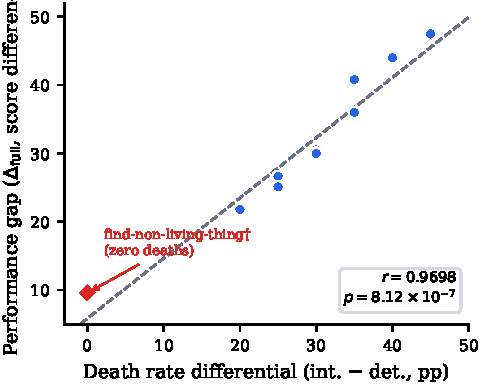
\includegraphics[width=0.75\columnwidth]{figures/fig1_daf_scatter.pdf}
\caption{Per-task death rate differential vs.\ performance gap ($n{=}11$ task types). The near-perfect correlation ($r = 0.97$) is a structural consequence of death dominance (DAF $\to 1 \Rightarrow r \to 1$), not an independent finding. The sole outlier (\texttt{find-non-living-thing}, red diamond) has zero deaths; its $\Delta_{\text{full}} = +9.58$ arises entirely from non-death score differences.}
\label{fig:decomposition}
\end{figure}

\paragraph{Per-task correlation structure.}
The internal strategy dies in 42.9\% of episodes versus 16.3\% for deterministic (2.6$\times$). Per-task death rate differential correlates with $\Delta_{\text{full}}$ ($r = 0.97$, $p < 10^{-6}$; Figure~\ref{fig:decomposition}); since DAF$\to 1$ implies $r \to 1$ by construction, the near-perfect correlation is a consistency check, not an independent finding (Appendix~\ref{app:correlation}). Of 245 episodes, 86 are \texttt{det\_preferred}, 9 \texttt{internal\_preferred}, and 150 \texttt{no\_preference}.

\paragraph{Signal concentration and binary structure.}
The Signal Concentration Index (SCI $= 0.2147$; Appendix~\ref{app:sci}) confirms low concentration: the top-3 task types account for only $39.8\%$ of total death-rate differential. The aggregate 78.9\% reflects a per-task binary structure: all 10 death-prone task types produce 100\% death-asymmetry labels, while \texttt{find-non-living-thing} (zero deaths, $\Delta = +9.58$ from non-death scores; case study in Appendix~\ref{app:non-death-case-study}) produces 0\%. The framework thus diagnoses a binary property (``is this environment death-dominated?'') rather than a continuous routing signal. A systematic decomposition of all 20 non-death labels (Appendix~\ref{app:non-death-case-study}) reveals they originate exclusively from this single task type, with hallucination-induced errors (50\%) dominating over object selection quality differences (35\%). Removing \texttt{find-non-living-thing} raises the label fraction to 100\% and yields DAF $\geq$100\% ($\Delta_\text{nd} \leq 0$; death avoidance fully accounts for the routing gap among remaining task types; Appendix~\ref{app:loto-daf}).

\paragraph{Sensitivity and seed robustness.}
Non-clustered episode-level bootstrap ($B = 10{,}000$) yields 95\% CI $[81.1\%, 99.0\%]$ for DAF; cluster-robust CI $[73.3\%, 100.0\%]$ ($K{=}11$; Appendix~\ref{app:wild-cluster}). Leave-one-task-out analysis confirms stability (label fraction range: 75.9\%--78.9\%; Appendix~\ref{app:loto-daf}); two independent replications---cross-model (Gemma-2-9B-it, DAF${}\,{=}\,89.7\%$; \S\ref{sec:cross-model}) and same-model with a different environment seed (seed=123, $N{=}220$, DAF${}\,{=}\,89.7\%$; Appendix~\ref{app:seed-robustness})---both converge within 0.7~pp. Exact permutation ($p=0.002$) and sign tests ($p<0.001$) on $K{=}11$ task-type clusters provide distribution-free confirmation (Appendix~\ref{app:wild-cluster}; supplementary evidence in Appendix~\ref{app:per-task-ci}).

\subsection{Multi-Model Validation (7--9B Tier)}
\label{sec:cross-model}

A Llama-3.1-8B-Instruct~\citep{llama3-2024} cross-model replication across all 11 task types ($N{=}220$) confirms that death dominance replicates across model families: internal death rate $41.4\%$ vs.\ deterministic $11.4\%$ (death-rate differential $+30.0$~pp), DAF $= 88.2\%$ (95\% CI: $[80.2\%, 95.1\%]$; $\Delta_{\text{full}} = +33.17$, $\Delta_{\text{nd}} = +3.9$), with direction consistency 10/10 on death-prone tasks, 83 deterministic-preferred, 3 internal-preferred (1.4\%, all death-asymmetry reversals), and 134 no-preference labels.
Both models show ${\sim}42\%$ internal vulnerability ($+26.5$ vs.\ $+30.0$~pp differential; per-task details in Appendix~\ref{app:cross-model}).
A third model family, Gemma-2-9B-it~\citep{gemma2-2024} (sliding window attention, vs.\ full attention in Qwen/Llama), independently confirms the pattern: DAF${=}89.7\%$ (95\% CI $[79.5\%, 98.4\%]$; $N{=}220$), with all 10 death-prone task types showing positive $\Delta$DR (Appendix~\ref{app:cross-model}). Three architecturally distinct models thus converge on DAF $88$--$90\%$ (spread 2.2~pp); $10{\times}$ scaling to 72B (\S\ref{sec:agent-improvement}) confirms persistence across capability levels (DAF${=}92.4\%$).

\subsection{Agent Improvement Baselines}
\label{sec:agent-improvement}

\begin{table}[t]
\centering
\small
\begin{tabular}{@{}lrr@{}}
\toprule
Condition & Death\% & $N$ \\
\midrule
Single-trial baseline & 42.9 & 245 \\
Reflexion ($3{\times}$) & 31.4 & 220 \\
Qwen2.5-72B ($10{\times}$) & 30.6 & 255 \\
Deterministic baseline & 16.3 & 245 \\
\midrule
\multicolumn{3}{@{}l}{\textit{10 death-prone tasks only:}} \\
Death-prone baseline & 48.0 & 200 \\
Retry ($5{\times}$) & 43.5 & 200 \\
\bottomrule
\end{tabular}
\caption{Internal-strategy death rates under agent improvement methods. Top: all 11 tasks (72B: independently collected at both internal and deterministic). Bottom: 10 death-prone tasks (\texttt{find-non-living-thing} excluded, 0\% death at all scales). All interventions reduce death rate but none approaches deterministic-level safety.}
\label{tab:agent-improvement}
\end{table}

We test whether agent-level improvement reduces death dominance (Table~\ref{tab:agent-improvement}). Retry ($N{=}5$ attempts without self-correction) yields marginal reduction on death-prone tasks ($43.5\%$ vs.\ $48.0\%$ baseline, $\Delta = -4.5$~pp). Reflexion~\citep{reflexion-2023}\footnote{Reflexion uses a fixed allocation of 20 episodes per task type ($20 \times 11 = 220$), vs.\ the baseline's variable 20--40 per type ($N{=}245$).} (verbal self-reflection between trials) reduces death to 31.4\% across all 11 tasks by rescuing 29.3\% of first-trial deaths, but the gap to deterministic remains 15.1~pp; on the 10 death-prone tasks, Reflexion achieves ${\sim}$35\%. Under Reflexion ($N{=}3$, matched-episode analysis), $\Delta_{\text{nd}} = -0.47$, yielding DAF $> 100\%$: the deterministic advantage is entirely attributable to death avoidance, and in non-death episodes the self-correcting agent slightly outperforms the deterministic baseline. As a preliminary probe, scaling to Qwen2.5-72B ($10{\times}$ parameters; both strategies independently collected at 72B, 255 episodes across all 11 task types) reduces death rate to $30.6\%$. The 72B deterministic strategy achieves $2.75\%$ death rate ($\Delta\text{DR} = +27.8$~pp), and $\Delta_{\text{nd}} = +2.28$, yielding DAF $= 92.4\%$ (95\% CI: $[86.1\%, 97.9\%]$; 7B: $90.4\%$), with 5 internal-preferred episodes (vs.\ 9 at 7B; $2.0\%$ vs.\ $3.7\%$). This $10{\times}$ scaling analysis (distinct from the 7--9B cross-family replication in \S\ref{sec:cross-model}) shows that while 72B reduces the internal death rate from $42.9\%$ to $30.6\%$, DAF \emph{increases} because the deterministic strategy also becomes safer ($2.75\%$ vs.\ $16.3\%$), making the proportional dominance of death avoidance more extreme.

\paragraph{Dose-response analysis.}
We extend both interventions to $N{=}5$ trials on death-prone tasks ($n{=}200$; Figure~\ref{fig:dose-response}). Retry is nearly flat ($48.0\% \to 43.5\%$). Reflexion drops steeply to $34.0\%$ at $N{=}3$ ($\Delta = -13.5$~pp, $p = 0.003$) then stabilizes ($34$--$36.5\%$ for $N \geq 3$, pairwise $p > 0.5$); both the decline and plateau are well-powered (MDE ${\sim}8$~pp at 80\% power; Appendix~\ref{app:dose-response}).

\begin{figure}[t]
\centering
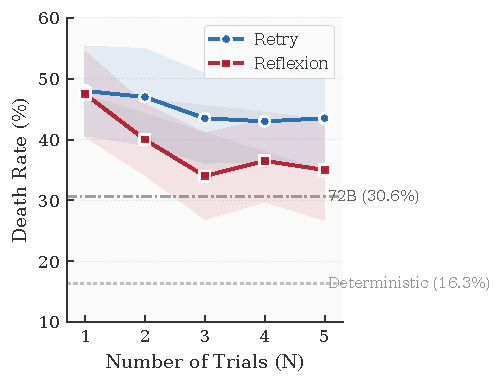
\includegraphics[width=\columnwidth]{figures/dose_response.pdf}
\caption{Death rate as a function of trial count ($N$) for Retry and Reflexion on 10 death-prone tasks ($n{=}200$). Retry (blue) is nearly flat; Reflexion (red) drops steeply through $N{=}3$ then shows no statistically detectable improvement beyond $N{=}3$ (Wilson CIs for $N{=}3,4,5$ overlap substantially). Horizontal lines: 72B scaling baseline ($30.6\%$) and deterministic baseline ($16.3\%$), both computed over all 11 task types; retry and Reflexion use 10 death-prone types only. Error bands: Wilson 95\% CIs.}
\label{fig:dose-response}
\end{figure}

\subsection{Cross-Environment Boundary Probes}
\label{sec:math-contrast}
\label{sec:cross-env}

We examine MATH and ALFWorld as boundary probes (not cross-domain validation). The deterministic oracle differs in information privilege across environments---ground-truth simulator (ScienceWorld), code interpreter (MATH), admissible-action enumeration (ALFWorld; \S\ref{sec:problem-setup})---so cross-environment results validate the diagnostic procedure's reusability, not the transferability of specific findings.

\paragraph{MATH.} On MATH Level~4--5~\citep{math-2021} ($N{=}795$, code interpreter), internal reasoning and code interpretation achieve near-identical accuracy ($73.5\%$ vs.\ $73.0\%$, McNemar $p = 0.81$), with 84.4\% no-preference. Without catastrophic failure, no routing signal emerges.

\paragraph{ALFWorld.} ALFWorld~\citep{alfworld-2021} (6 task types, 135 games) provides the deterministic strategy with admissible actions, an information asymmetry rather than a computation mode switch, with no death mechanism ($\delta = 0$, DAF $= 0\%$). With Qwen2.5-7B, 35 of 37 non-tie labels (94.6\%) favor the information-advantaged strategy (Appendix~\ref{app:cross-env-details}); Llama-3.1-8B (135 games) yields 16 of 16 non-tie labels in the same direction (100\%). Llama shows fewer non-tie episodes (11.9\% vs.\ 25.9\%) but perfect directional consistency, confirming that information asymmetry, not death avoidance, drives routing signal in ALFWorld regardless of model family. The framework diagnoses this qualitatively different mechanism (DAF $= 0\%$ vs.\ $90.4\%$) without modification.

\subsection{Baselines}
\label{sec:baselines}

\begin{table}[t]
\centering
\small
\resizebox{\columnwidth}{!}{%
\begin{tabular}{@{}lccc@{}}
\toprule
Strategy & Score & 95\% CI & Death \% \\
\midrule
Always-Internal & $-39.07$ & [$-46.40$, $-32.27$] & 42.9 \\
Always-Deterministic & $-9.47$ & [$-14.71$, $-4.29$] & 16.3 \\
Random & $-22.38$ & [$-28.67$, $-15.75$] & 27.8 \\
Oracle & $-6.58$ & [$-11.54$, $-1.70$] & 14.3 \\
\midrule
Trained Router$^\dagger$ & $-10.70$ & [$-16.33$, $-5.27$] & 17.6 \\
\bottomrule
\end{tabular}}
\caption{Episode-weighted mean scores on ScienceWorld (11 task types, 20--40 episodes per type, 245 total). $\dagger$\,Single random seed (42) per episode pair; see Appendix~\ref{app:seed-robustness} for 8-seed robustness analysis. Per-task results are exploratory ($n{=}20$ episodes per task, power $\approx 50\%$ for 20\,pp effects); aggregate conclusions do not depend on individual task significance.}
\label{tab:baselines}
\end{table}

Always-deterministic ($-9.47$) outperforms always-internal ($-39.07$) by 29.60 points. The oracle improves only to $-6.58$, with 96.3\% of decisions matching always-deterministic---an \emph{oracle degeneracy} where an always-deterministic lookup achieves 90.5\% of non-tie oracle decisions (balanced accuracy 50.0\%: perfect deterministic recall, zero internal recall).

\subsection{Router Training: Inconclusive Results}
\label{sec:router-diagnostic}

We probe whether counterfactual labels can train a step-level router, as a diagnostic of label informativeness. The oracle margin (2.89 points) caps routing upside. An implicit router (Qwen3, LoRA; Appendix~\ref{app:router-details}) trained at three scales (0.6B, 1.7B, 4B) shows flat step-level balanced accuracy ($56$--$59\%$); episode-level independent evaluation yields $47.1 \pm 2.2\%$, below the majority-vote baseline.\footnote{The near-chance performance is consistent with noisy-label learning bounds~\citep{natarajan2013learning,northcutt2021confident}: ${\sim}$88\% of step-level labels are uninformative, class imbalance is extreme (90.5\% deterministic-preferred, 3.7\% minority), and paraphrase-based text augmentation (25\%--800\%) provides no improvement (Appendix~\ref{app:seed-robustness}).} Leave-one-task-type-out analysis degrades to chance (49.2\%; Appendix~\ref{app:ablations}), as does a task-type-only classifier ($64.7\%$ in-distribution, $50.0\%$ LOTO), confirming routing signal is a per-task-type constant with no cross-type generalization. Deployed end-to-end, the best router scores $-10.70$ (95\% CI: $[-16.33, -5.27]$), not exceeding always-deterministic ($-9.47$). Results remain inconclusive under the current data regime ($N{=}245$, 3.7\% minority class).
